% -*- Mode:TeX -*-

%% IMPORTANT: The official thesis specifications are available at:
%%            http://libraries.mit.edu/archives/thesis-specs/
%%
%%            Please verify your thesis' formatting and copyright
%%            assignment before submission.  If you notice any
%%            discrepancies between these templates and the 
%%            MIT Libraries' specs, please let us know
%%            by e-mailing thesis@mit.edu

%% The documentclass options along with the pagestyle can be used to generate
%% a technical report, a draft copy, or a regular thesis.  You may need to
%% re-specify the pagestyle after you \include  cover.tex.  For more
%% information, see the first few lines of mitthesis.cls. 

%\documentclass[12pt,vi,twoside]{mitthesis}
%%
%%  If you want your thesis copyright to you instead of MIT, use the
%%  ``vi'' option, as above.
%%
%\documentclass[12pt,twoside,leftblank]{mitthesis}
%%
%% If you want blank pages before new chapters to be labelled ``This
%% Page Intentionally Left Blank'', use the ``leftblank'' option, as
%% above. 

\documentclass[12pt,vi,twoside]{mitthesis}
\usepackage{lgrind}
%% These have been added at the request of the MIT Libraries, because
%% some PDF conversions mess up the ligatures.  -LB, 1/22/2014
\usepackage{cmap}
\usepackage[T1]{fontenc}
\pagestyle{headings}

%% This bit allows you to either specify only the files which you wish to
%% process, or `all' to process all files which you \include.
%% Krishna Sethuraman (1990).

\typein [\files]{Enter file names to process, (chap1,chap2 ...), or `all' to
process all files:}
\def\all{all}
\ifx\files\all \typeout{Including all files.} \else \typeout{Including only \files.} \includeonly{\files} \fi

\begin{document}

% -*-latex-*-
% 
% For questions, comments, concerns or complaints:
% thesis@mit.edu
% 
%
% $Log: cover.tex,v $
% Revision 1.8  2008/05/13 15:02:15  jdreed
% Degree month is June, not May.  Added note about prevdegrees.
% Arthur Smith's title updated
%
% Revision 1.7  2001/02/08 18:53:16  boojum
% changed some \newpages to \cleardoublepages
%
% Revision 1.6  1999/10/21 14:49:31  boojum
% changed comment referring to documentstyle
%
% Revision 1.5  1999/10/21 14:39:04  boojum
% *** empty log message ***
%
% Revision 1.4  1997/04/18  17:54:10  othomas
% added page numbers on abstract and cover, and made 1 abstract
% page the default rather than 2.  (anne hunter tells me this
% is the new institute standard.)
%
% Revision 1.4  1997/04/18  17:54:10  othomas
% added page numbers on abstract and cover, and made 1 abstract
% page the default rather than 2.  (anne hunter tells me this
% is the new institute standard.)
%
% Revision 1.3  93/05/17  17:06:29  starflt
% Added acknowledgements section (suggested by tompalka)
% 
% Revision 1.2  92/04/22  13:13:13  epeisach
% Fixes for 1991 course 6 requirements
% Phrase "and to grant others the right to do so" has been added to 
% permission clause
% Second copy of abstract is not counted as separate pages so numbering works
% out
% 
% Revision 1.1  92/04/22  13:08:20  epeisach

% NOTE:
% These templates make an effort to conform to the MIT Thesis specifications,
% however the specifications can change.  We recommend that you verify the
% layout of your title page with your thesis advisor and/or the MIT 
% Libraries before printing your final copy.
%\title{SCE16-0446\\
% Time-Dependent Shortest Path Queries on Mobile Devices}
\title{SCE16-0446\\
A Machine Learning-Based Approach to Time-Dependent Shortest Path Queries}


\author{Wei Yumou}
% If you wish to list your previous degrees on the cover page, use the 
% previous degrees command:
%       \prevdegrees{A.A., Harvard University (1985)}
% You can use the \\ command to list multiple previous degrees
%       \prevdegrees{B.S., University of California (1978) \\
%                    S.M., Massachusetts Institute of Technology (1981)}

\department{School of Computer Science and Engineering}

% If the thesis is for two degrees simultaneously, list them both
% separated by \and like this:
% \degree{Doctor of Philosophy \and Master of Science}
\degree{Bachelor of Computer Science}

% As of the 2007-08 academic year, valid degree months are September, 
% February, or June.  The default is June.
\degreemonth{June}
\degreeyear{2017}
\thesisdate{\today}


%% By default, the thesis will be copyrighted to MIT.  If you need to copyright
%% the thesis to yourself, just specify the `vi' documentclass option.  If for
%% some reason you want to exactly specify the copyright notice text, you can
%% use the \copyrightnoticetext command.  
%\copyrightnoticetext{\copyright IBM, 1990.  Do not open till Xmas.}

% If there is more than one supervisor, use the \supervisor command
% once for each.
\supervisor{Xiao Xiaokui}{Associate Professor, Assistant Chair (Strategic Research)}


% This is the department committee chairman, not the thesis committee
% chairman.  You should replace this with your Department's Committee
% Chairman.
\chairman{abc}{abc}


% Make the titlepage based on the above information.  If you need
% something special and can't use the standard form, you can specify
% the exact text of the titlepage yourself.  Put it in a titlepage
% environment and leave blank lines where you want vertical space.
% The spaces will be adjusted to fill the entire page.  The dotted
% lines for the signatures are made with the \signature command.
\maketitle
%\pagestyle{empty}

% The abstractpage environment sets up everything on the page except
% the text itself.  The title and other header material are put at the
% top of the page, and the supervisors are listed at the bottom.  A
% new page is begun both before and after.  Of course, an abstract may
% be more than one page itself.  If you need more control over the
% format of the page, you can use the abstract environment, which puts
% the word "Abstract" at the beginning and single spaces its text.

%% You can either \input (*not* \include) your abstract file, or you can put
%% the text of the abstract directly between the \begin{abstractpage} and
%% \end{abstractpage} commands.

% First copy: start a new page, and save the page number.
\cleardoublepage
% Uncomment the next line if you do NOT want a page number on your
% abstract and acknowledgments pages.
%\pagestyle{empty}
\setcounter{savepage}{\thepage}
\begin{abstractpage}
% $Log: abstract.tex,v $
% Revision 1.1  93/05/14  14:56:25  starflt
% Initial revision
% 
% Revision 1.1  90/05/04  10:41:01  lwvanels
% Initial revision
% 
%
%% The text of your abstract and nothing else (other than comments) goes here.
%% It will be single-spaced and the rest of the text that is supposed to go on
%% the abstract page will be generated by the abstractpage environment.  This
%% file should be \input (not \include 'd) from cover.tex.
In this thesis, I designed and implemented a compiler which performs
optimizations that reduce the number of low-level floating point operations
necessary for a specific task; this involves the optimization of chains of
floating point operations as well as the implementation of a ``fixed'' point
data type that allows some floating point operations to simulated with integer
arithmetic.  The source language of the compiler is a subset of C, and the
destination language is assembly language for a micro-floating point CPU.  An
instruction-level simulator of the CPU was written to allow testing of the
code.  A series of test pieces of codes was compiled, both with and without
optimization, to determine how effective these optimizations were.

\end{abstractpage}

% Additional copy: start a new page, and reset the page number.  This way,
% the second copy of the abstract is not counted as separate pages.
% Uncomment the next 6 lines if you need two copies of the abstract
% page.
% \setcounter{page}{\thesavepage}
% \begin{abstractpage}
% % $Log: abstract.tex,v $
% Revision 1.1  93/05/14  14:56:25  starflt
% Initial revision
% 
% Revision 1.1  90/05/04  10:41:01  lwvanels
% Initial revision
% 
%
%% The text of your abstract and nothing else (other than comments) goes here.
%% It will be single-spaced and the rest of the text that is supposed to go on
%% the abstract page will be generated by the abstractpage environment.  This
%% file should be \input (not \include 'd) from cover.tex.
In this thesis, I designed and implemented a compiler which performs
optimizations that reduce the number of low-level floating point operations
necessary for a specific task; this involves the optimization of chains of
floating point operations as well as the implementation of a ``fixed'' point
data type that allows some floating point operations to simulated with integer
arithmetic.  The source language of the compiler is a subset of C, and the
destination language is assembly language for a micro-floating point CPU.  An
instruction-level simulator of the CPU was written to allow testing of the
code.  A series of test pieces of codes was compiled, both with and without
optimization, to determine how effective these optimizations were.

% \end{abstractpage}

\cleardoublepage


\section*{Acknowledgments}

I would like to express my sincere gratitude to my supervisor, Assoc Prof. Xiao Xiaokui, who gave me this great opportunity to work on GPS trajectory mining and offered valuable insights to help me tackle challenges. 

I would also like to thank my parents and friends who have been constantly providing me with lots of emotional support. 

Lastly, I would appreciate the Computational Sensing Lab at Tsinghua University, Beijing, China, for their generosity in sharing the data set used in this project and also thank Baidu for providing wonderful Baidu Maps APIs which constitute an essential part of this project. 
%%%%%%%%%%%%%%%%%%%%%%%%%%%%%%%%%%%%%%%%%%%%%%%%%%%%%%%%%%%%%%%%%%%%%%
% -*-latex-*-

% Some departments (e.g. 5) require an additional signature page.  See
% signature.tex for more information and uncomment the following line if
% applicable.
% % -*- Mode:TeX -*-
%
% Some departments (e.g. Chemistry) require an additional cover page
% with signatures of the thesis committee.  Please check with your
% thesis advisor or other appropriate person to determine if such a 
% page is required for your thesis.  
%
% If you choose not to use the "titlepage" environment, a \newpage
% commands, and several \vspace{\fill} commands may be necessary to
% achieve the required spacing.  The \signature command is defined in
% the "mitthesis" class
%
% The following sample appears courtesy of Ben Kaduk <kaduk@mit.edu> and
% was used in his June 2012 doctoral thesis in Chemistry. 

\begin{titlepage}
\begin{large}
This doctoral thesis has been examined by a Committee of the Department
of Chemistry as follows:

\signature{Professor Jianshu Cao}{Chairman, Thesis Committee \\
   Professor of Chemistry}

\signature{Professor Troy Van Voorhis}{Thesis Supervisor \\
   Associate Professor of Chemistry}

\signature{Professor Robert W. Field}{Member, Thesis Committee \\
   Haslam and Dewey Professor of Chemistry}
\end{large}
\end{titlepage}


\pagestyle{headings}
  % -*- Mode:TeX -*-
%% This file simply contains the commands that actually generate the table of
%% contents and lists of figures and tables.  You can omit any or all of
%% these files by simply taking out the appropriate command.  For more
%% information on these files, see appendix C.3.3 of the LaTeX manual. 
\tableofcontents
\newpage
\listoffigures
\newpage
\listoftables


%% This is an example first chapter.  You should put chapter/appendix that you
%% write into a separate file, and add a line \include{yourfilename} to
%% main.tex, where `yourfilename.tex' is the name of the chapter/appendix file.
%% You can process specific files by typing their names in at the 
%% \files=
%% prompt when you run the file main.tex through LaTeX.
\chapter{Introduction}

Finding a practically shortest route on a large road network in a metropolis is not only of algorithmic interests, but also of economic and environmental values. Less travelling time means less fuel consumptions and less carbon emissions. However, finding shortest routes can be challenging, especially when the road traffic is known to be \emph{time-dependent} or \emph{dynamic}, namely, when the road conditions change with respect to time. It may take 10 minutes on average to traverse a particular road at 10a.m, but it is possible that the expected travel time increases to 20 minutes at 5p.m. Moreover, two different roads may have different time-varying patterns. For instance, one road may have a peak traveling time at 12p.m but the other may have two peaks at 8 a.m. and 6 p.m., respectively.

The formal definition of a dynamic road network is given as follows.
\begin{defn}[\emph{Dynamic road network}]
A dynamic road network is a weighted, directed graph $G=(V,E)$ where $E$ represents a set of road segments and $V$ denotes the set of intersections of these road segments. It has a weight function $w : E,t \rightarrow \mathbb{R}$, where $t$ represents an instant in time. 
\end{defn}
With the definition of a dynamic road network, the generalised time-dependent shortest path problem can be formally defined as follows.
\begin{defn}[\emph{Generalised time-dependent shortest path problem}]
In a dynamic road network $G=(V,E)$, given a source node $u$, a destination node $v$ and a departure time $t$ from $u$, find a path $p$ that satisfies:
\begin{equation}
w(p)=\delta(u,v)=
\begin{cases}
\text{min}\left\{w(p): u\overset{p}{\leadsto}v \right\} &\text{if there is a path from $u$ to $v$,}\\
\infty &\text{otherwise.}
\end{cases}
\end{equation}
where $w(p)$ is the weight of the path $p$ and defined as sum of the weights of its constituent edges, and $\delta(u,v)$ is called the \textbf{shortest-path weight} from $u$ to $v$.
\end{defn}

A typical Bellman-Ford\cite{CLRS09} or Dijkstra's algorithm\cite{Dij59} for finding shortest paths assume the cost of traversing each edge in the abstract graph is constant with respect to time and therefore, do not work on time-de\-pendent road networks without appropriate modifications. Fortunately, most online mapping services such as Google Maps or Apple Maps are able to recommend shortest routes by incorporating real-time traffic information. This project seeks to investigate an alternative approach of finding shortest routes on a dynamic road network based on mining a GPS\footnote{Global Positioning System} trajectory database aggregated from thousands of taxis in Beijing, China.

Chapter two describes the preliminary data processing. Chapter three introduces the approach for building a landmark graph. Chapter four explains how to estimate the travel time for each landmark graph edge. Chapter five presents methods for evaluating travel time estimations. 

\section{Motivations for mining taxi GPS trajectories}
Taxi drivers or any experienced car drivers, more often than not, possess some \emph{implicit} knowledge or intuitions about which route from source $u$ to destination $v$ is the best in terms of travelling time at a particular moment. Such knowledge or intuitions come from everyday experiences. For example, a taxi driver may observe that there are always traffic jams during 6 p.m. to 7 p.m. on a particular street and hence avoids travelling on that street during that period whenever possible. But observations of this kind, albeit valuable, are just too subtle to be captured by any general algorithms and oftentimes, even the drivers themselves may not be aware of that.

However, mining their GPS trajectories can reveal such knowledge to some extent. In a metropolis such as Beijing or New York, taxi drivers are required by regulations to install GPS devices on their cars and to send time-stamped GPS information to a central reporting agency periodically for management and security reasons. Such information typically includes latitudes, longitudes, instantaneous speeds and heading directions. Therefore, the GPS data is readily available and little effort is needed to collect it. By means of mapping to a real road network all GPS data points of a particular taxi during a specific period of time, a GPS trajectory can be obtained to represent the driver's intelligence. 

\section{Practical limitations} \label{Sec:limitation}
There are some practical limitations that are worth mentioning. 
\subsubsection{Arbitrary sources and destinations}
In a typical map-query use case, a user is able to select an arbitrary source to start with and an arbitrary destination to go to. But this may not be possible in the GPS-based approach, since the taxi GPS trajectories do not necessarily cover every part of a city's map. It is likely that there are no trajectories passing through the source and the destination.
\subsubsection{Low sampling rate}
Taxis report their locations to the central reporting agency at a relatively low rate to conserve energy. For the data set used in this project, the expected sampling interval is one minute. But oftentimes, the GPS device may not be working properly or may be occasionally shut down due to various reasons, which causes the actual sampling interval to fluctuate. 

Even if the sampling interval \emph{is} strictly kept at one minute, for a taxi moving at a typical speed of $60km/h$, it means the distance between two consecutive sample points is $1km$. Such a large distance increases the uncertainty of the \emph{exact} trajectory that the taxi has moved along. The picture\cite{TDR10} below demonstrates a problem caused by low sampling rate and long inter-sample-point distance.
\begin{figure}[h]
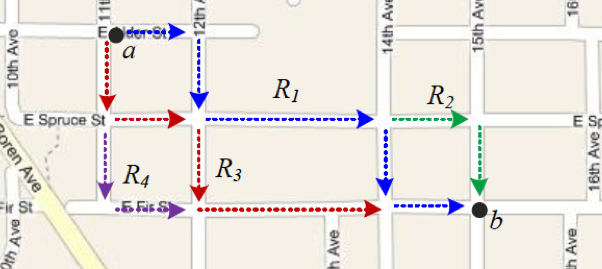
\includegraphics{low_sample_rate}
\centering
\caption{Example of low sampling rate problem}
\end{figure}

The taxi is known to have traversed from point $a$ to point $b$. But there are four possible trajectories from $a$ to $b$. The exact route cannot be determined without additional information in this case.
\subsubsection{Limited GPS accuracy}
After decades of development, the GPS service has achieved great accuracy, but it is still not completely error-free. A report\cite{FP15} in 2015 showed that GPS-enabled smartphones typically have an accuracy of 5 metres \emph{under open sky}. But in a metropolis like Beijing, the actual accuracy may be lower than this value due to the reflection of signals amongst high buildings. Moreover, the data set used in this project was collected in 2009 when GPS devices had lower accuracy than that of today's.

The limited accuracy in GPS devices makes the exact mapping from a GPS data point to a street impossible. In Beijing, there is usually a side road running in parallel with a main road. Due to that limited accuracy, the taxi might be \emph{actually} on the side road but the GPS data point is shown on the main road, or vice versa. 

\section{Related work}
The incentive for carrying out this project comes from a similar project\cite{TDR10}, and similar procedures are followed in this project but with some modifications. 



\chapter{Preliminary Data Processing}
\section{Data Collection and Cleaning}
The taxi GPS data used in this project is collected from the Computational Sensing Lab\cite{BPLL13} at Tsinghua University, Beijing, China. The data set contains approximately 83 million time-stamped taxi GPS records collected from 8,602 taxis in Beijing, from 1 May 2009 to 30 May 2009. The original data set consists of seven fields as shown in Table~\ref{Ta:orig_field}. Longitude and latitude in the data set are defined in the WGS-84\footnote{World Geodetic System} standard coordinate system, which is the reference coordinate system used by the GPS.

\begin{table}
\centering
\begin{tabular}{ | l | l | l | }
\hline
\textbf{Field} & \textbf{Explanation} \\ \hline
CUID & ID for each taxi \\ \hline
UNIX\_EPOCH & Unix timestamp in milliseconds since 1 January 1970\\ \hline
GPS\_LONG & Longitude encoded in WGS-84 multiplied by $10^{5}$\\ \hline
GPS\_LAT & Latitude encoded in WGS-84 multiplied by $10^{5}$ \\ \hline
HEAD & Heading direction in degrees with 0 denoting North\\ \hline
SPEED & Instantaneous speed in metres/second (m/s)\\ \hline
OCCUPIED & Binary indicator of whether the taxi is hired (1) or not (0)\\ \hline
\end{tabular}
\caption{Fields in the original data set}\label{Ta:orig_field}
\end{table}

The original data set came in a binary file format. After the data set was decoded and imported into a MySQL database, the first step in data cleaning was \textbf{to delete all records with zero value in the SPEED field}, since when a taxi is stationary it yields no valuable information about the \emph{trajectory} it is moving along. While being stationary could be due to a traffic jam, this kind of information is well captured by the time difference between the last \emph{non-stationary} data point and the next \emph{non-stationary} data point. 

In addition, all records must have a \emph{unique} pair of CUID and UNIX\_EPOCH fields, since it is not possible for a taxi to appear in two different locations at the same moment in time. This kind of error is likely due to some errors in aggregating the original data set.

\section{Reverse Geocoding}
After the data set was cleaned, the next step was to map each GPS data point to a road segment, which is also known as \emph{reverse geocoding}. A number of algorithms\cite{MAP09} have been proposed for this purpose, but most of them require an additional GIS\footnote{Geographic Information System} database of the road network in Beijing. This project adopted an alternative strategy which leveraged on the existing public APIs\footnote{Application Programming Interface} for reverse geocoding. 

Currently, a number of online mapping platforms provide reverse geocoding services as part of their developer APIs. Amongst others, Google Maps and Baidu Maps offer relatively stable and fast reverse geocoding services. However, due to the ``China GPS shift problem''\cite{GSHF17} where coordinates encoded in WGS-84 format are required by regulations to be shifted by a large and variable amount when displayed on a street map, Google Maps is not able to display a GPS data point correctly because it only supports WGS-84 formats. Figure~\ref{Fig:gps_shift} illustrates the effect of such shift, with the correct location displayed on the right. 

\begin{figure}[h]
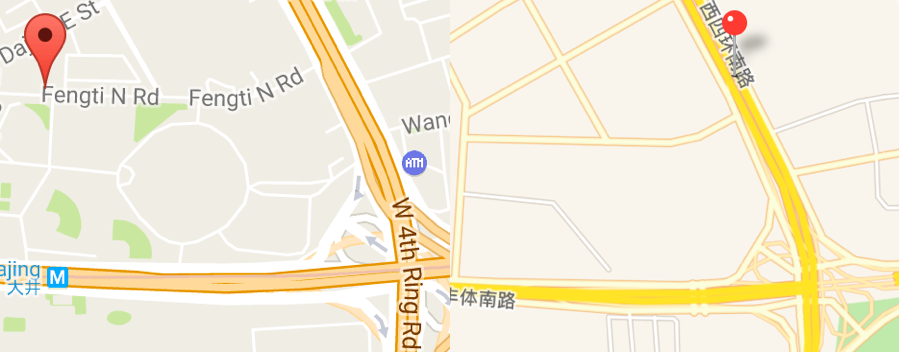
\includegraphics{gps_shift}
\centering
\caption{China GPS shift problem}\label{Fig:gps_shift}
\end{figure}

Baidu Maps, on the other hand, has been using their own coordinate system, BD-09, which is an improved version of the Chinese official coordinate system, GCJ-02. Baidu provides a set of APIs to convert WGS-84 coordinates into BD-09 ones. Therefore, to reverse-geocode the data points, the coordinates must be converted to BD-09 format. To store the converted coordinates as well as the street names obtained from reverse geocoding, four new fields were added to the original data set as shown in Table~\ref{Ta:addtional_field}.

\begin{table}
\centering
\begin{tabular}{ | l | l | l | }
\hline
\textbf{Field} & \textbf{Explanation} \\ \hline
DataUnitID & Nominal primary key for each record \\ \hline
UTC & UNIX\_EPOCH in human readable format \\ \hline
BD09\_LONG & Longitude encoded in BD-09 format\\ \hline
BD09\_LAT & Latitude encoded in BD-09 format\\ \hline
STREET & Street name\\ \hline
\end{tabular}
\caption{Additional fields added to data set}\label{Ta:addtional_field}
\end{table}

In order to use Baidu APIs for coordinate conversion, the following system architecture was set up as shown in Figure~\ref{Fig:basic_architecture}. The Apache HTTP server hides the MySQL database and sends HTTP POST request to Baidu Maps Web API to get converted coordinates. Then it updates the database through PHP \emph{mysqli} utilitity. 

\begin{figure}[h]
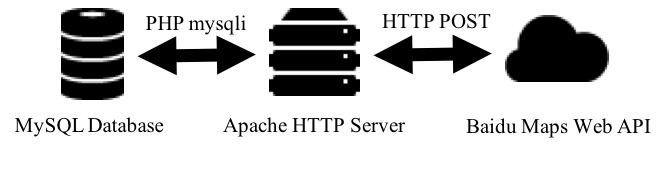
\includegraphics{basic_architecture}
\centering
\caption{Basic system architecture}\label{Fig:basic_architecture}
\end{figure}

After the coordinates were converted from WGS-84 format to BD-09 format, Baidu Maps Web API was used to reverse geocode all GPS data points. However, the system architecture was slightly changed, to accommodate the change in technology used. For reverse geocoding, AJAX\footnote{Asynchronous JavaScript and XML} was used to communicate with the Baidu Maps Web API for speed and unlimited number of requests per day. Therefore, one additional layer was added to the existing system architecture as shown in Figure~\ref{Fig:ajax_architecture}. 

\begin{figure}[h]
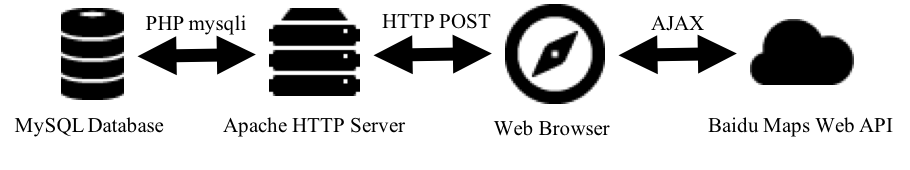
\includegraphics{ajax_architecture}
\centering
\caption{Augmented system architecture}\label{Fig:ajax_architecture}
\end{figure}

Executed in a web browser environment, AJAX sent HTTP POST requests to the Apache HTTP server to fetch the converted coordinates in BD-09 format which were subsequently sent to the Baidu Maps Web API server \emph{asynchronously} via HTTP GET requests. Once the server responded with the name of the road segment, AJAX updated the database by sending another HTTP POST request to the Apache HTTP server. The asynchronous nature of this architecture, however, caused a few problems which are addressed in Section~\ref{outlier_detecting}. 

\section{Outlier Detection}\label{outlier_detecting}
\subsection{Motivation for Outlier Detection}
The Baidu Maps Web API for reverse geocoding is stable and fast, but does not produce no errors. Sometimes, a GPS data point may be mapped to a main road but actually it is on the side road, which is one of the limitations mentioned in Section~\ref{Sec:limitation} or it is actually mapped to a street that Baidu Maps does not recognise. In neither case will Baidu Maps produce a correct reverse geocoding. Moreover, the reverse geocoding process is asynchronous, which means that it is being performed in the background in parallel with the main application thread. Therefore, it is inevitable that some street names may get lost when the records are being updated or a record is updated with a wrong street name. Figure~\ref{Fig:exmp_outlier} shows a drastic example.

\begin{figure}[h]
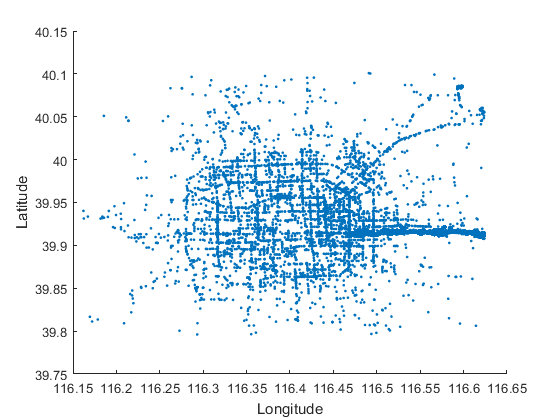
\includegraphics{long_lat_plot}
\centering
\caption{Example of outliers}\label{Fig:exmp_outlier}
\end{figure}

In this example, the Baidu Maps believes that all data points plotted belong to a particular street. But when plotted on a 2-D plane, these data points almost represent the \emph{entire} road network in Beijing. The actual, correct street is represented in the figure as the \emph{thickest} line on the right half of the figure with a longitude ranging from 116.45\textdegree~to 116.65\textdegree.~Erroneous records like those not on the thickest line are known as \emph{outliers} and must be properly identified and removed. This project proposes a novel outlier detection approach based on unsupervised learning whose principle behind is based on Theorem~\ref{Theorem: majority_clustering}.

\begin{defn}[\emph{Reasonable reverse geocoder}]\label{Def:reasonable_geocoder}
A reasonable reverse geocoder always gives its best matching from a GPS data point to a street whenever possible and has an accuracy more than 50\%.
\end{defn}

\begin{theorem}[\emph{Majority Clustering Theorem}]\label{Theorem: majority_clustering}
If a \emph{reasonable reverse geocoder} is used to reverse geocode a set of GPS data points which are mapped to a particular street \emph{in reality}, then, when plotted on a 2-D plane, majority (more than 50\%) of the points must be clustered together to form a rough shape that is similar to the shape of the street that they are supposed to be mapped to. 
\end{theorem}

\begin{proof}
Proof by contradiction. Assume, for the purpose of contradiction, majority (more than 50\%) of the data points that are \emph{indeed} located on the same street are scattered arbitrarily on a 2-D plane after being reverse-geocoded by a reasonable reverse geocoder. In particular, when plotted on a 2-D plane, majority of them do not form a similar shape to that of the street they are supposed to be mapped to. Then, the majority must have been erroneously mapped to some other streets because no single street covers the whole city area. Thus, the reasonable reverse geocoder has only achieved an accuracy less 50\%, which contradicts the Definition~\ref{Def:reasonable_geocoder} of a reasonable reverse geocoder. 
\end{proof}

\subsection{Outlier Identification}\label{SubSec:outlier_identify}
Apparently, Baidu Maps provides a reasonable reverse geocoder because it is of industrial-grade quality and has an accuracy larger than 50\%. Therefore, if a set of points belong to a particular street, after reverse-geocoded by Baidu Maps, majority of them should be clustered to assume a rough shape of that street according to Theorem~\ref{Theorem: majority_clustering}. Based on that, an unsupervised learning technique --- clustering can be used to separate the correctly mapped data points from outliers. 

Many clustering techniques are available\cite{LO05}. Since each record can be represented graphically by a point on a 2-D plane with longitute as the $x$ axis and latitude as the $y$ axis, a \textbf{self-organising feature map}\cite{TK82}(SOFM) seems to be an appropriate technique to use. 

\begin{figure}[h]
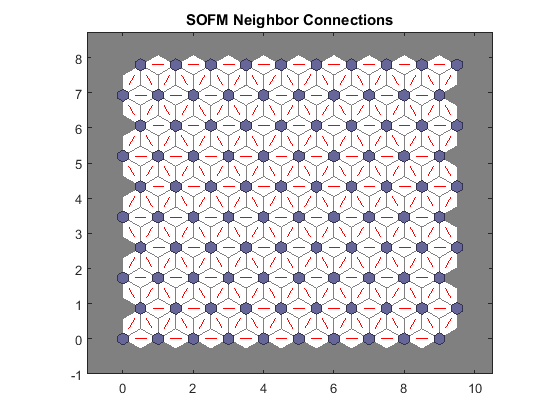
\includegraphics{neighbour_connections}
\centering
\caption{An example of SOFM}\label{Fig:neighbour_connections}
\end{figure}

A self-organising feature map is a form of artificial neural network. It consists of a pre-defined number of interconnected neurons distributed over a 2-D plane as shown in Figure~\ref{Fig:neighbour_connections}. Prior to training, the neurons are randomly scattered among the data points and gradually move to the centroids of the data clusters they represent as they learn the \emph{features} of the training data. Upon termination of the training, all data points near to a particular neuron, in terms of Euclidean distance\footnote{Other distance measures are also possible.}, are assigned to the cluster that neuron represents. Figure~\ref{Fig:sofm_weights} shows the results after the clustering is completed. 

\begin{figure}[h]
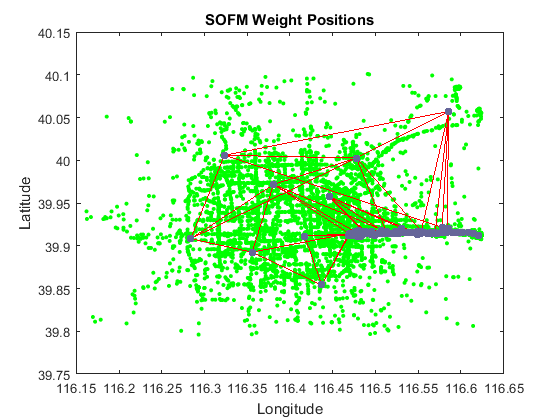
\includegraphics{sofm_weights}
\centering
\caption{Neuron positions after training}\label{Fig:sofm_weights}
\end{figure}

It is clear from the figure that while some neurons represent the clusters of outliers, majority of the neurons are clustered to \emph{cover} the correct street they should represent. A $10\times10$ SOFM was used in this project, so there were at most 100 neurons or equivalently, 100 clusters. Each cluster had a different size. To ensure a thorough removal of the outliers, \textbf{only the top 50\% largest clusters were considered as clusters of correct data points which are called ``legal clusters''. All other clusters were deemed as clusters of outliers}. 

\subsection{Outlier Removal}\label{Subsec:outlier_removal}
Once the legal clusters were identified, a distance threshold was set to remove outliers so that \textbf{whenever the minimum distance between a data point and all centroids of the legal clusters was above the threshold, that data point would be considered as an outlier and removed}. The python-like pseudocode in Listing~\ref{List:code_outlier} describes this idea with more clarity.

%\begin{minipage}{\linewidth}
\begin{lstlisting}[language = Python, caption = {Pseudocode for outlier detection}, label = {List:code_outlier} ,frame=single, numbers=left,stepnumber=1]
for record in records:
	min_distance = math.inf // infinity
	for centroid in centroids:
		min_distance = min(min_distance, \
			get_distance(record, centroid))
	if min_distance > threshold:
		remove(records, record)
\end{lstlisting}
%\end{minipage}

However, the \emph{distance} between a data point and a centroid is not as straightforward as Euclidean distance. A centroid, to some extent, can be imagined as a \emph{real} point on the Earth's surface. To calculate the distance between a data point and a centroid is to calculate the spherical distance which is given by the haversine formula in Theorem~\ref{Theorem: haversine}. 

\begin{theorem}[\emph{Haversine Formula}]\label{Theorem: haversine}
Given two points $P(\lambda_1,\varphi_1)$ and $Q(\lambda_2,\varphi_2)$ on the surface of a sphere, where $\lambda$ and $\varphi$ represent longitude and latitude in radians, their spherical distance (the distance along a great circle of the sphere) is given by\cite{FI06}
\begin{equation}
d = 2R\arcsin{\sqrt{\sin^2\frac{\varphi_2 - \varphi_1}{2} + \cos\varphi_1\cos\varphi_2\sin^2\frac{\lambda_2 - \lambda_1}{2}}} 
\end{equation}
where $R$ is the radius of the sphere. 
\end{theorem}

Since the Earth is not a perfect sphere, $R$ varies with latitude. Theorem~\ref{Theorem: radius_latitide} suggests how to calculate the Earth radius at any latitude. 

\begin{theorem}[\emph{Radius at any Latitude}]\label{Theorem: radius_latitide}
Given a latitude $\varphi$ in radians, a polar radius $R_{p}$ and an equatorial radius $R_{e}$, the spheroid's radius at that latitude is given by\cite{EAR17}
\begin{equation}
R(\varphi) = \sqrt{\frac{(R_{e}^2\cos\varphi)^2 + (R_{p}^2\sin\varphi)^2}{(R_{e}\cos\varphi)^2 + (R_{p}\sin\varphi)^2}}
\end{equation}
\end{theorem}

It is known that $R_{e} = 6,378,137$ metres and $R_{p} = 6,356,752$ metres on the Earth\cite{NASA16} and that Beijing's latitude is about 39\textdegree N. Therefore, the distance between a data point and a centroid can be calculated. For this project, two thresholds were selected: 30 metres and 50 metres. The thresholds were set in a way that it ensured there was sufficient data for subsequent machine learning tasks while the estimates were as least affected as possible by outliers. If the threshold were set to a too small value, the remaining data could not have been sufficient; on the other hand, however, if the threshold were set to a too big value, the accuracy of the final results would have been subject to outliers. 

\begin{figure}[h]
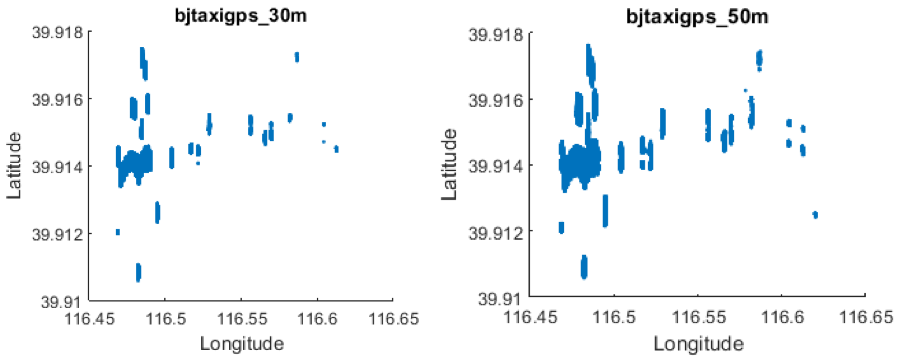
\includegraphics{30m_50m}
\centering
\caption{Plot of data points after outlier removal}\label{Fig:after_removal}
\end{figure}

After the outliers were removed, two data sets remained. They are hereinafter referred to as \emph{bjtaxigps\_30m}, where outliers were filtered by a threshold of 30 metres and \emph{bjtaxigps\_50m}, where outliers were filtered by a threshold of 50 metres, respectively. bjtaxigps\_30m contains approximately 51 million records while bjtaxigps\_50m has 59 million. All algorithms described hereinafter are applicable to both data sets. Figure~\ref{Fig:after_removal} gives a plot of the data points from both data sets. Clearly, the data points are now contained in a much smaller area and roughly form a shape similar to that of the street they are mapped to. 
\appendix
\chapter{Source Code}
\section{Database Utilities}
The source code listed in this section provides utility functions for general database operations, such as \textbf{select} and \textbf{update}. It is to be used in other modules. 

\begin{lstlisting}[language = PHP, caption = {Database Utilities}, label = {AList:db_utilities}, frame=single, numbers=left, stepnumber=1]
<?php
include "../inc/jingodbinfo.inc";

function connect_db(){
    $conn = new mysqli(DB_SERVER, DB_USERNAME, DB_PASSWORD);
    if($conn->connect_error){
	die("Connection failed: " . $conn->connect_error);
    }
    $conn->select_db(DB_DATABASE);
    $conn->set_charset("utf8");
    return $conn;
}

function disconnect_db($conn){ $conn->close(); }

function db_select($conn, $table, $cols, $cond = "true", $distinct = "")
{
    $sql_select = "SELECT {$distinct} ";
    if(count($cols) == 0){
        $sql_select .= "*,";
    }
    foreach ($cols as $col) {
        $sql_select .= "{$col},";
    }
    $sql_select = rtrim($sql_select, ",");
    $sql_select .= " FROM {$table} WHERE {$cond};";
    $ret = $conn->query($sql_select);
    $res = array();
    if($ret->num_rows > 0){
        while($row = $ret->fetch_assoc()){
            $curr = array();
            foreach ($cols as $col) {
                $curr[$col] = $row[$col];
            }
            $res[] = $curr;
	}
    }
    return $res;
}

function db_update($conn, $table, $values, $cond){
    $sql_update = "UPDATE {$table} SET ";
    foreach ($values as $key => $value) {
        if(is_numeric($value)){
            $sql_update .= "{$key} = {$value},";
        }else{
            $sql_update .= "{$key} = '{$value}',";
        }
    }
    $sql_update = rtrim($sql_update, ",");
    $sql_update .= " WHERE {$cond};";
    $succ = $conn->query($sql_update);
    return $succ;
}

function db_insert($conn, $table, $values, $cond = "", $ignore = ""){
    $sql_insert = "INSERT {$ignore} INTO {$table} ";
    $cols = "";
    $vals = "";
    foreach ($values as $key => $value) {
        $cols .= "{$key},";
        $vals .= (is_numeric($value) ? "{$value}," : "'{$value}',");
    }
    $cols = rtrim($cols, ",");
    $vals = rtrim($vals, ",");
    $sql_insert .= "({$cols}) VALUES ({$vals}) {$cond};";
    echo "{$sql_insert}\n";
    $conn->query($sql_insert);
}

function db_delete($conn, $table, $cond){
    $sql_delete = "DELETE FROM {$table} WHERE {$cond};";
}
?>
\end{lstlisting}

\clearpage
\newpage

\section{Data Pre-processing}
This section lists down the source code used in data pre-processing. 

\begin{lstlisting}[language = PHP, caption = {Outlier Removal}, label = {AList:outlier_rmvl}, frame=single, numbers=left, stepnumber=1]
<?php
include "db_utilities.php";

class Filter{
    private $ldmk_start;
    private $ldmk_end;
    private $ldmk_table;
    private $data_table;
    private $update_table;
    private $path;
    private $bchmk;
    
    private $conn;
    private $num_dele;
    
    public function __construct($ldmk_start, $ldmk_end, $ldmk_table, $data_table, $path, $bchmk, $update_table){
        $this->ldmk_start = $ldmk_start;
        $this->ldmk_end = $ldmk_end;
        $this->ldmk_table = $ldmk_table;
        $this->data_table = $data_table;
        $this->update_table = $update_table;
        $this->path = $path;
        $this->bchmk = $bchmk;
        $this->conn = connect_db();
        $this->num_dele = 0;
    }
    
    public function __destruct(){ disconnect_db($this->conn); }
    
    private function getCentres($ldmk){
        $filename = "{$this->path}{$ldmk}.csv";
        $centres = array();
        if(($handle = fopen($filename, 'r')) !== FALSE){
            while(($line = fgetcsv($handle, 0, ',')) !== FALSE){
                $centres[] = array($line[0], $line[1]);
            }
	}
	return $centres;
    }
    
    private function getRecords($ldmk){
        $ldmk_cols = array('LandmarkName');
        $ldmk_cond = "LandmarkID = {$ldmk}";
        $ret = db_select($this->conn, $this->ldmk_table, $ldmk_cols, $ldmk_cond);
        $data_cols = array('DataUnitID', 'BD09_LONG', 'BD09_LAT');
        $data_cond = "Street = '{$ret[0][$ldmk_cols[0]]}'";
        $ret = db_select($this->conn, $this->data_table, $data_cols, $data_cond);
        $records = array();
        foreach ($ret as $item) {
            $records[] = array($item[$data_cols[0]], $item[$data_cols[1]], $item[$data_cols[2]]);
        }
        return $records;
    }
    
    
    private function removeRecord($centres, $records){
        foreach ($records as $recd) {
            $min_dist = INF;
            foreach ($centres as $centre) {
                $min_dist = min($min_dist, $this->getHaversineDist
                ($centre[0], $centre[1], $recd[1], $recd[2]));
            }
            if($min_dist > $this->bchmk){
                $cond = "DataUnitID = {$recd[0]}";
                db_delete($this->conn, $this->data_table, $cond);
                ++$this->num_dele;
            }
	}
    }
    
    private function toRadian($degree){ return $degree * M_PI / 180; }
    
    private function getHaversineDist($long1, $lat1, $long2, $lat2){
        $BJ_LAT = $this->toRadian(39);
        $EQ_R = 6378137; // equatorial radius in metres
        $POL_R = 6356752; // polar radius in metres

	$BJ_R = sqrt((pow($EQ_R * $EQ_R * cos($BJ_LAT), 2) + pow($POL_R * $POL_R * sin($BJ_LAT), 2)) / (pow($EQ_R * cos($BJ_LAT), 2) + pow($EQ_R * sin($BJ_LAT), 2)));
	$long1 = $this->toRadian($long1);
	$lat1 = $this->toRadian($lat1);
	$long2 = $this->toRadian($long2);
	$lat2 = $this->toRadian($lat2);
	$d = 2 * $BJ_R * asin(sqrt(pow(sin(($lat1 - $lat2) / 2), 2) + 
	cos($lat1) * cos($lat2) * pow(sin(($long1 - $long2) / 2), 2)));
	return $d; }
    private function getWithin($ldmk, $centres, $records){
        foreach ($records as $recd) {
	    $min_dist = INF;
	    foreach ($centres as $centre) {
	        $min_dist = min($min_dist, 
		$this->getHaversineDist($centre[0], $centre[1], $recd[1], $recd[2]));
	    }
	    if($min_dist <= $this->bchmk){
	        db_insert($this->conn, $this->update_table, 
			array('LandmarkID' => $ldmk, 'BD09_LONG' => $recd[1], 'BD09_LAT' => $recd[2]));
	    }
	}
    }
    
    public function doFiltering(){
	for($ldmk = $this->ldmk_start; $ldmk != $this->ldmk_end; 
		++$ldmk){
	    $centres = $this->getCentres($ldmk);
	    $records = $this->getRecords($ldmk);
	    $this->getWithin($ldmk, $centres, $records);
	}
    }
}
set_time_limit(0);
ini_set('memory_limit','2048M');
$filter = new Filter($_POST['ldmk_start'], $_POST['ldmk_end'], 
	$_POST['ldmk_table'], $_POST['data_table'], $_POST['path'], 
	$_POST['bchmk'], $_POST['update_table']);
$filter->doFiltering();
?>
\end{lstlisting}

\chapter{Figures}

\vspace*{-3in}

\begin{figure}
\vspace{2.4in}
\caption{Armadillo slaying lawyer.}
\label{arm:fig1}
\end{figure}
\clearpage
\newpage

\begin{figure}
\vspace{2.4in}
\caption{Armadillo eradicating national debt.}
\label{arm:fig2}
\end{figure}
\clearpage
\newpage

%\bibliography{main}
%\bibliographystyle{alpha}
%% This defines the bibliography file (main.bib) and the bibliography style.
%% If you want to create a bibliography file by hand, change the contents of
%% this file to a `thebibliography' environment.  For more information 
%% see section 4.3 of the LaTeX manual.
\begin{singlespace}
\bibliography{main}
\bibliographystyle{plain}
\end{singlespace}

\end{document}

